% *==================================================================================*
% *                     Review vs. Camera-Ready settings                             *
% *==================================================================================*
%
% REVIEW: Use the following command for submitting the paper (double-blind,
% for review):
% \documentclass{Interspeech}
%
% CAMERA-READY: Use the following command for the camera-ready version, one
% affiliation per line:
\documentclass[cameraready]{Interspeech}
%\documentclass{Interspeech}
\def\argmax{\mathop{\rm argmax}}

% *==================================================================================*


% **************************************
% *                                    *
% *      STOP !   DO NOT DELETE !      *
% *          READ THIS FIRST           *
% *                                    *
% * This template also includes        *
% * important INSTRUCTIONS that you    *
% * must follow when preparing your    *
% * paper. Read it BEFORE replacing    *
% * the content with your own work.    *
% **************************************

%==================================================================================
% Title
% Must exactly match the title entered into the paper submission system
%\title{Speculative Decoding for LLM-based ASR Using Draft CTC Predictions}
\title{Self-Speculative Decoding for LLM-based ASR with CTC Encoder Drafts}

%==================================================================================
% Authors
% The order of authors here must exactly match the order entered into the paper submission system
% Note that the COMPLETE list of authors MUST be entered into the paper submission system at the outset, including when submitting your manuscript for double-blind review
% The ORCID number is still optional but will become mandatory in the future years. It is strongly encouraged to get an ORCID for each cu-author.
% Middle names, including initials, must be included in the first name
\author{George}{Saon}
\author{Samuel}{Thomas}
\author{Takashi}{Fukuda}
\author{Tohru}{Nagano}
\author{Avihu}{Dekel}
\author{Luis}{Lastras}
% The maximum number of authors in the author list is 20. If the number of contributing authors is more than this, they should be listed in a footnote or the acknowledgement section.

%==================================================================================
% Affiliations

\address{
    IBM Research
}

%==================================================================================
% Emails
\email{gsaon@us.ibm.com}

%==================================================================================
% Keywords
\keywords{speech recognition, speech-aware LLM, speculative decoding}

\newcommand{\blue}[1]{\textcolor{blue}{#1}}
\newcommand{\red}[1]{\textcolor{red}{#1}}
\usepackage{comment}
\usepackage{diagbox}
\usepackage{multirow}
\usepackage{colortbl}

%==================================================================================
% Content

\begin{document}

\maketitle

% the abstract here must exactly match the abstract entered into the paper submission system
\begin{abstract}
    % 1000 characters. ASCII characters only. No citations.
We propose self-speculative decoding for speech-aware LLMs by using the CTC encoder as a draft model to accelerate auto-regressive (AR) inference and improve ASR accuracy. Our three-step procedure works as follows: (1) if the frame entropies of the CTC output distributions are below a threshold, the greedy CTC hypothesis is accepted as final; (2) otherwise, the CTC hypothesis is verified in a single LLM forward pass using a relaxed acceptance criterion based on token likelihoods; (3) if verification fails, AR decoding resumes from the accepted CTC prefix. Experiments on nine corpora and five languages show that this approach can simultaneously accelerate decoding and reduce WER. On the HuggingFace Open ASR benchmark with a 1B parameter LLM and 440M parameter CTC encoder, we achieve a record 5.58\% WER and improve the inverse real time factor by a factor of 4.4 with only a 12\% relative WER increase over AR search. Code and model weights are publicly available under a permissive license.
    
\end{abstract}

\section{Introduction}

As a special case of attention encoder-decoder (AED) models~\cite{chan2016listen}, speech-aware language models (short SLMs) are currently the best performing ASR systems in terms of recognition accuracy. Indeed, the top five open models on the HuggingFace Open ASR leaderboard~\cite{srivastav2025open} are SLMs with similar architectures. They all use conformer acoustic encoders trained with either RNN-T loss~\cite{rekesh2023fast,sekoyan2025canary}, CTC loss~\cite{saon2025granite}, or with next token cross-entropy loss as part of an AED ASR model~\cite{abouelenin2025phi,shi2026qwen3asrtechnicalreport} and speech modality adapters which are either MLPs~\cite{chen2024salm,abouelenin2025phi} or query transformers~\cite{saon2025granite}. The role of the adapters is to perform a temporal downsampling and to project the acoustic embeddings coming out of the encoder to a space that is interpretable by the LLM. For ASR, the LLM is trained to perform a repetition-like task~\cite{grattafiori2024llama} in the sense that the embeddings of the output tokens can be seen as denoised versions of the speech embeddings. 

One of the main drawbacks of AED models and, by extension, of SLMs is that inference is done auto-regressively, one token at a time, which requires one forward pass through the text LLM per generated token. This limits parallelism compared to non-autoregressive approaches where output tokens are predicted simultaneously such as CTC with greedy decoding, CTC with mask-predict error correction~\cite{higuchi2020mask} or iterative realignment~\cite{chi2021align}. Another class of models which have a good accuracy / inference speed tradeoff, termed semi-autoregressive, predict multiple output tokens at once within blocks of frames~\cite{arora2024semi} or jointly predict tokens and durations~\cite{xu2023efficient}. 

Accelerating AR inference for text LLMs via speculative decoding is an active area of research. In~\cite{leviathan2023fast} and~\cite{chen2023accelerating}, the authors use a small draft AR model that runs in parallel to the large target model and produces $K$ future tokens at a time conditioned on the current hypothesis which get verified by the target model in a single forward pass. If the verification fails, the target model falls back to AR decoding from the first position where the draft and target model distributions differ. The main idea in self speculative decoding is to reuse the target model itself as a draft model either by simultaneously predicting tokens at future positions $i+1\ldots i+N$ with $N$ separate LM heads as in ~\cite{cai2024medusa} or by using predictions from intermediate layers (early exit)~\cite{zhang2024draft}. 

An application of speculative decoding to ASR for transformer-based encoder-decoders is discussed in~\cite{lim2025hybrid} where the authors train a small token and duration transducer (TDT)~\cite{xu2023efficient} decoder together with the frozen encoder which serves as a draft model for the larger causal transformer decoder. There are several differences between~\cite{lim2025hybrid} and our proposed work. First, we reuse the CTC encoder of the SLM instead of training a separate decoder for the draft model. Second, the authors focus on mitigating repetition errors whereas we show that complementary error patterns between CTC and SLM can actually improve WER. Third, we use a confidence metric given by the frame-level entropies of the CTC output distributions~\cite{laptev2023fast} which allows skipping SLM verification entirely for confident CTC hypotheses.

Other techniques that are relevant to our work are two-pass approaches that use a fast model for the first pass such as RNN-T or AR and either rescore candidate hypotheses~\cite{sainath2019two} or refine the output with a slower AR model~\cite{hu2020deliberation}, and joint CTC/attention models with score fusion during inference~\cite{watanabe2017hybrid}. 

As to limitations of our proposed approach, we note that: (1) it requires an SLM with a CTC-trained encoder that is frozen during projector training and LoRA finetuning of the LLM; (2) our technique is limited to ASR and is not applicable to other speech tasks like translation or spoken question answering; (3) the SLM verification of the CTC hypothesis is utterance-based meaning that, if verification fails, the entire utterance has to be AR-decoded from the failed verification point\footnote{While it is possible to dynamically rejoin the CTC draft through local DP, we found this approach to be inefficient for batched inference.} which limits the gains for corpora with low acceptance rates. We mitigate (3) by using a relaxed acceptance criterion which requires the CTC hypothesis to be {\em plausible} under the SLM distribution instead of an exact match of the SLM verification hypothesis.  

The paper is organized as follows: in section~\ref{sec:method} we describe our proposed method, in section~\ref{sec:experiments} we show some experimental evidence of its utility, and in section~\ref{sec:conclusion} we summarize our findings and propose future directions.

\begin{figure*}[t]                                                                                                                                                                       \centering                                                                                                                                                                               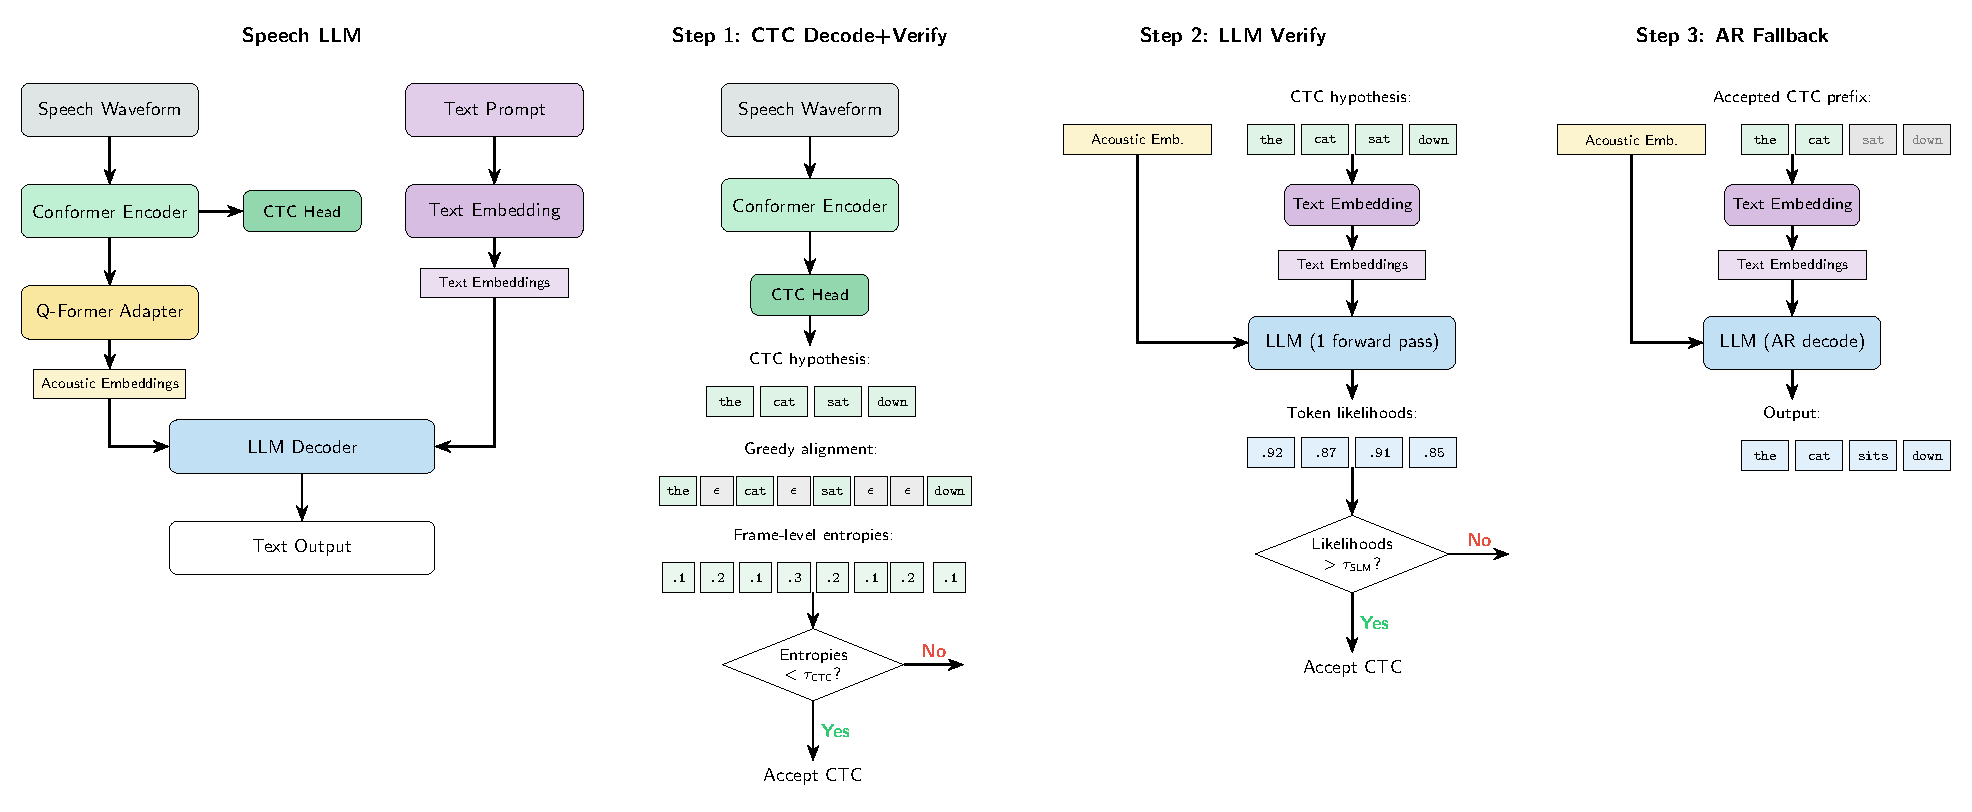
\includegraphics[width=\textwidth]{figures/cascade_figure.pdf}                                                                                                                                   \caption{Overview of the proposed self-speculative decoding method for speech-aware LLMs.}                                                                                               \label{fig:cascade}                                                                                                                                                                      \end{figure*}                                                                                                                                                                                                       
\section{Method description}
\label{sec:method}
In this section we describe our method in detail specifically the CTC decoding and verification pass (subsection~\ref{subsec:CTC}), the SLM verification pass (subsection~\ref{subsec:SLM-verif}), and the SLM auto-regressive fallback pass (subsection~\ref{subsec:SLM-AR}). The three steps as well as the chosen SLM architecture are illustrated in Figure~\ref{fig:cascade}.
\subsection{CTC decoding and verification}
\label{subsec:CTC}
In order to introduce some notations, we recall that the CTC formulation~\cite{graves2006connectionist} models the conditional distribution $p_{CTC}({\bf y}|{\bf x})$ of an output sequence  ${\bf y}=(y_1,\ldots,y_U)\in{\cal Y}^*$ of length $U$ given an input
sequence ${\bf x}=(x_1,\ldots,x_T)\in{\cal X}^*$ of length $T\ge U$. The
elements of ${\bf x}$ are continuous multidimensional
vectors whereas the elements of ${\bf y}$ belong to a discrete output space. $p({\bf y}|{\bf x})$ is expressed as a
sum over all possible alignments ${\bf a}=(a_1,\ldots,a_{T})$ that
are consistent with ${\bf y}$:

\begin{equation}
p_{CTC}({\bf y}|{\bf x})=\sum_{{\bf a}\in{\cal B}^{-1}({\bf y})}p({\bf a}|{\bf x})=\sum_{{\bf a}\in{\cal B}^{-1}({\bf y})}\prod_{t=1}^T p(a_t|h_t)
\label{ll}
\end{equation}
~~\\
where ${\bf h}=(h_1,\ldots,h_T)=Encoder({\bf x})$ is a sequence of acoustic embeddings computed by an encoder and the elements of ${\bf a}$ belong to the augmented vocabulary
$\overline{{\cal Y}}={\cal Y}\cup\{\epsilon\}$ where $\epsilon$ (called blank) denotes the null output. ${\cal B}$ is a mapping that removes consecutive duplicates and blanks (in this order) such that ${\cal B}({\bf a})={\bf y}$. We compute the draft CTC hypothesis as $\hat{{\bf y}} = {\cal B}(\hat{{\bf a}})$ with

\begin{equation}
\hat{{\bf a}}=(\hat{a}_1,\ldots,\hat{a}_T)=(\argmax_{a\in\overline{{\cal Y}}}p(a|h_1),\ldots,\argmax_{a\in\overline{{\cal Y}}}p(a|h_T))
\end{equation}
~~\\
denoting the greedy alignment path. The draft hypothesis is accepted as final if all the frame-level entropies of the CTC output distribution are less than a threshold i.e.

\begin{equation}
\sum_{a\in\overline{\cal Y}}-p(a|h_t)\log p(a|h_t) < \tau_{CTC}\qquad\forall t\in\{1,\ldots,T\}
\label{eq:CTC-verif}
\end{equation}

\subsection{SLM verification of the CTC hypothesis}
\label{subsec:SLM-verif}
In comparison to~(\ref{ll}), SLMs model the conditional distribution of the output sequence ${\bf y}$ given the input sequence ${\bf x}$ differently:
\begin{equation}
p_{SLM}({\bf y}|{\bf x})=\prod_{i=1}^U p(y_i|{\bf y}_{<i},{\bf x})=\prod_{i=1}^U p(y_i|{\bf y}_{<i},{\bf g})
\end{equation}
~~\\
where ${\bf g}=(g_1,\ldots,g_{T'})=Adapter({\bf h})$, $T'\le T$, is a sequence of LLM-compatible acoustic embeddings computed by a speech modality adapter that takes as input the embedding sequence ${\bf h}$ computed by the CTC encoder. The draft CTC hypothesis $\hat{\bf y}$ is accepted during the SLM verification pass if all the token likelihoods under the SLM output distribution are greater than a threshold:

\begin{equation}
p(\hat{y}_i|\hat{{\bf y}}_{<i},{\bf g}) > \tau_{SLM}\qquad\forall i\in\{1,\ldots,|\hat{\bf y}|\}
\label{eq:SLM-verif}
\end{equation}

Note that, because of the causal attention mask of the text LLM,~(\ref{eq:SLM-verif}) can be computed in parallel for all tokens with a single forward pass through the LLM. The reason why we use entropy in~(\ref{eq:CTC-verif}) and likelihood in~(\ref{eq:SLM-verif}) is because the specific hypothesis $\hat{{\bf y}}$ needs to be verified for the latter.  

\subsection{Auto-regressive fallback pass with CTC prefix}
\label{subsec:SLM-AR}
If~(\ref{eq:SLM-verif}) does not hold, we find the longest verified CTC prefix $\hat{{\bf y}}_{<j}$ where $j=\min\{i\in\{1,\ldots,|\hat{\bf y}|\}~s.t.~p(\hat{y}_i|\hat{{\bf y}}_{<i},{\bf g}) \le \tau_{SLM}\}$ and simply continue auto-regressive generation from there:

\begin{equation}
\overline{\bf y}=\argmax_{{\bf y}\in{\cal Y}^*}p_{SLM}({\bf y}|\hat{{\bf y}}_{<j},{\bf x})
\end{equation}
~~\\
In summary, the final hypothesis that is output by the self-speculative decoding (short SSD) process is

\begin{equation}
{\bf y}_f=\left\{
\begin{array}{ll}
\hat{\bf y}, &\mathrm{if}~(\ref{eq:CTC-verif})~\mathrm{or}~(\ref{eq:SLM-verif})\\
(\hat{{\bf y}}_{<j},\overline{\bf y}),&\mathrm{otherwise}
\end{array}
\right.
\end{equation}

 \begin{table}[!t]                                                                                                                                                                                                           
    \centering                                                                                                                                                                                                                
    \caption{Comparing full AR and self-speculative decoding for granite-speech-4.0-1b. High accuracy: $\tau_{\text{CTC}}\!=\!0.7, \tau_{\text{SLM}}\!=\!0.2$. High RTFx: $\tau_{\text{CTC}}\!=\!3.0,                         
  \tau_{\text{SLM}}\!=\!0.1$.  \%C/\%L = CTC/LLM acceptance rates at each verification stage. RTFx are measured on 1 H100. $^{*}p<0.0001$, $^{\dagger}p<0.05$ (Statistical significance was assessed using two-proportion z-test).}                 
    \label{tab:results}                                                                                                                                                                                                       
    \footnotesize                                                                                                                                                                                                             
    \setlength{\tabcolsep}{3pt}
    %\begin{tabular}{@{}l rr rrrr rr@{}}
    \begin{tabular}{@{}l rr rr@{\hspace{3pt}}r@{\hspace{3pt}}r rr@{}}
    \toprule                                                                                                                                                                                                                  
    & \multicolumn{2}{c}{\textbf{Full AR}} & \multicolumn{4}{c}{\textbf{High Accuracy}} & \multicolumn{2}{c}{\textbf{High RTFx}} \\                                                                                           
    \cmidrule(lr){2-3} \cmidrule(lr){4-7} \cmidrule(lr){8-9}                                                                                                                                                                  
    \textbf{Test set} & WER & RTFx & WER & RTFx & \%C & \%L & WER & RTFx \\                                                                                                                                                   
    \midrule                                                                                                                                                                                                                  
    \multicolumn{9}{@{}l}{\textit{English (Open ASR)}} \\                                                                                                                                                                     
    AMI\_IHM    & 8.65 & 455 & 8.31 & 621 & 39 & 39 & 9.40 & 1716 \\                                                                                                                                                          
    Earnings22  & 9.19 & 391 & 8.96 & 278 &  6 & 19 & 11.44& 1982 \\                                                                                                                                                          
    GigaSpeech  &10.19 & 511 & 9.95 & 514 & 10 & 51 & 10.67& 2503 \\                                                                                                                                                          
    LS Clean    & 1.37 & 510 & 1.37 & 712 & 17 & 73 & 1.63 & 2160 \\                                                                                                                                                          
    LS Other    & 3.02 & 476 & 2.88 & 667 & 18 & 61 & 3.77 & 2108 \\                                                                                                                                                          
    SPGISpeech  & 3.97 & 666 & 3.80 & 592 &  6 & 44 & 4.48 & 2736 \\                                                                                                                                                          
    Tedlium     & 3.38 & 358 & 3.35 & 444 &  9 & 60 & 3.91 & 1748 \\                                                                                                                                                          
    VoxPopuli   & 6.21 & 304 & 5.99 & 365 & 12 & 51 & 7.18 & 2035 \\                                                                                                                                                          
    \rowcolor{gray!15}                                                                                                                                                                                                        
    \textbf{Avg.} & \textbf{5.75} & \textbf{564} & \textbf{5.58}\rlap{$^{*}$} & \textbf{548} & 14 & 47 & \textbf{6.56} & \textbf{2491} \\                                                                                          
    \midrule                                                                                                                                                                                                                  
    \multicolumn{9}{@{}l}{\textit{Multilingual (MLS)}} \\                                                                                                                                                                     
    MLS En      & 4.74 & 702 & 4.72 & 772 &  1 & 42 & 5.75 & 2983 \\                                                                                                                                                          
    MLS De      & 4.59 & 663 & 4.42 & 755 &  3 & 48 & 4.91 & 2755 \\                                                                                                                                                          
    MLS Es      & 3.28 & 627 & 3.22 & 779 &  3 & 50 & 3.66 & 2490 \\                                                                                                                                                          
    MLS Fr      & 4.51 & 634 & 4.48 & 658 &  1 & 39 & 5.52 & 2834 \\                                                                                                                                                          
    MLS Pt      &10.25 & 521 & 9.84 & 531 &  8 & 10 & 8.83 & 2701 \\                                                                                                                                                          
    \rowcolor{gray!15}                                                                                                                                                                                                        
    \textbf{Avg.} & \textbf{5.47} & \textbf{629} & \textbf{5.33}\rlap{$^{\dagger}$} & \textbf{699} & 3 & 38 & \textbf{5.73} & \textbf{2753} \\                                                                                             
    \midrule                                                                                                                                                                                                                  
    \multicolumn{9}{@{}l}{\textit{Multilingual (CommonVoice)}} \\                                                                                                                                                             
    CV En       & 6.52 & 954 & 6.56 & 716 & 28 & 31 & 9.30 & 2446 \\                                                                                                                                                          
    CV De       & 4.79 & 872 & 4.71 & 998 &  0 & 59 & 6.34 & 2309 \\                                                                                                                                                          
    CV Es       & 4.04 & 752 & 3.98 & 890 &  1 & 59 & 5.42 & 2526 \\                                                                                                                                                          
    CV Fr       & 7.15 & 674 & 7.10 & 910 &  0 & 46 & 10.69& 2341 \\                                                                                                                                                          
    CV Pt       & 2.82 & 866 & 2.80 &1066 &  5 & 69 & 3.83 & 2344 \\                                                                                                                                                          
    \rowcolor{gray!15}                                                                                                                                                                                                        
    \textbf{Avg.} & \textbf{5.06} & \textbf{824} & \textbf{5.03} & \textbf{916} & 7 & 53 & \textbf{7.11} & \textbf{2393} \\                                                                                          
    \bottomrule                                                                                                                                                                                                               
    \end{tabular}                                                                                                                                                                                                             
  \end{table}
\begin{figure}
\centering
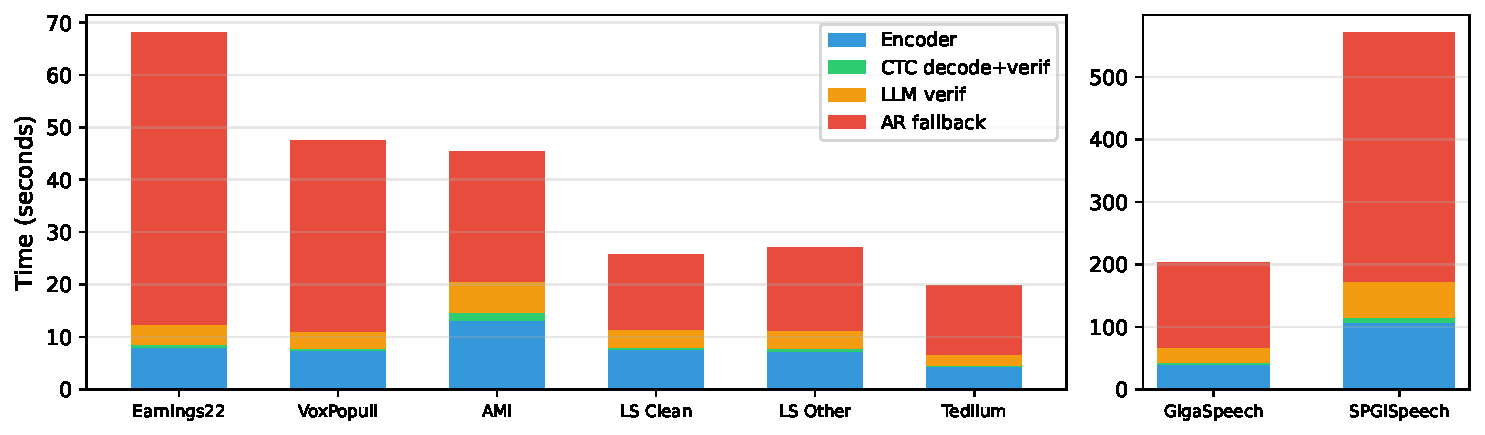
\includegraphics[width=8cm]{figures/timing_breakdown.pdf}
\caption{Run times and breakdown for the different passes in the high accuracy SSD regime for granite-speech-4.0-1b.}
\label{fig:timing}
\end{figure}                                                        

\section{Experiments and results}
\label{sec:experiments}
We selected Granite Speech~\cite{saon2025granite} as the SLM for our experiments because it satisfies the constraint of having a frozen acoustic encoder trained with CTC and has shown excellent performance on the Open ASR leaderboard~\cite{srivastav2025open}. We report results for the existing granite-speech-3.3-2b and granite-speech-3.3-8b models as well as a newly trained SLM on top of a 1B parameter granite-4.0-nano LLM~\cite{granite2025}. We discuss the architecture and training specifics for the latter in terms of training and evaluation data, encoder architecture and CTC training, followed by projector architecture and training with LLM finetuning.

%What needs to be done:\\
% WER-RTFx for 3.3-2b, 3.3-8b, 4.0-1b AR, 4.0-1b speculative, canary-qwen and parakeet\\
%- WER-RTFx ablation for deactivating CTC verif and LLM verif pass\\
%- detailed results for high-accuracy and high-throughput settings (WER, RTFx, acceptance \%, prefix length)\\
%- heat map for the influence of tau\_CTC and tau\_SLM\\
%- break down of where the time is spent in high-acc and high-RTFx mode

\subsection{Data, architecture and training specifics}
Our model is trained on 90,000 hours of data from major publicly available multilingual ASR datasets in English, French, German, Spanish, Portuguese and Japanese as well as bidirectional synthetic translations of CommonVoice to and from English to support the speech translation task. Concretely, our CTC encoder is trained on Multilingual LibriSpeech~\cite{pratap2020mls}, CommonVoice 17.0~\cite{ardila2019common}, LibriSpeech~\cite{panayotov2015librispeech}, Voxpopuli~\cite{wang2021voxpopuli}, AMI~\cite{kraaij2005ami}, YODAS~\cite{li2023yodas}, Earnings-22~\cite{delrio2022earnings22} (train partition cf.~\cite{gandhi2022esbbenchmarkmultidomainendtoend}), Switchboard~\cite{godfrey1992switchboard}, CallHome, Fisher~\cite{cieri2004fisher}, Voicemail~\cite{padmanabhan2002automatic} and ReazonSpeech~\cite{yin2023reazonspeech}. Projector training and LLM finetuning use the previously mentioned corpora plus 21,000 hours of synthetic translation data using Phi-4~\cite{abdin2024phi}, MADLAD~\cite{kudugunta2023madlad} and Granite 3~\cite{granite2024granite}  translations. We also report ASR results on Gigaspeech~\cite{chen2021gigaspeech}, SPGI Speech~\cite{o2021spgispeech} and TED LIUM~\cite{rousseau2012ted} which were excluded from our training data because of non-commercial licenses.

The 440M parameter encoder consists of 16 conformer layers of hidden dimension 1024 with 4-second block self-attention and conditioning on intermediate predictions from the middle layer. The output layer of size 348 contains the first 256 ASCII character entries to cover the European languages plus 92 Katakana phonetic characters for Japanese. It was trained with character-level CTC on all the ASR corpora specified previously for 20 epochs with a batch size of 256 using a mix of balanced and natural distribution sampling. 

We use a two-layer 37M parameter query transformer (q-former) projector that downsamples the acoustic embeddings by a factor of 5 for every window of 15 consecutive frames using 3 trainable queries per layer~\cite{tang2023salmonn}. The initial 10ms 80-dimensional log-mel frames are temporally downsampled by a factor of 10 (2x from the encoder, 5x from the projector). The projector and rank-64 LoRA adapters for the linear LLM modules are trained jointly for 3 epochs, 900k updates, with a peak learning rate of 1e-4 and a batch size of 128 utterances on all the corpora mentioned before using balanced sampling.

\subsection{Experimental details}
For all experiments, we measure WER and inverse real-time factor (RTFx = audio duration divided by processing time) on 1 H100 in a batched decoding setting using bfloat16 precision. To saturate the GPU, we sort the utterances by audio length and use adaptive batching controlled by a maximum number of tokens (set to 50K in practice) and perform separate batching for the CTC+LLM verification phases and the AR fallback phase with CPU-offloading of the acoustic embeddings for the utterances that fail verification between the passes. Additional optimizations include: (1) merging LoRA parameters and LLM weights to avoid LoRA computation overhead; (2) separate instantiation of the LLM for granite-speech to enable flash attention (FA2) since granite-speech does not support FA2 natively; (3) computing LLM logits only at CTC verification positions instead of the entire prompt that includes the text instruction and acoustic embeddings.

\begin{figure}[!t]
\centering
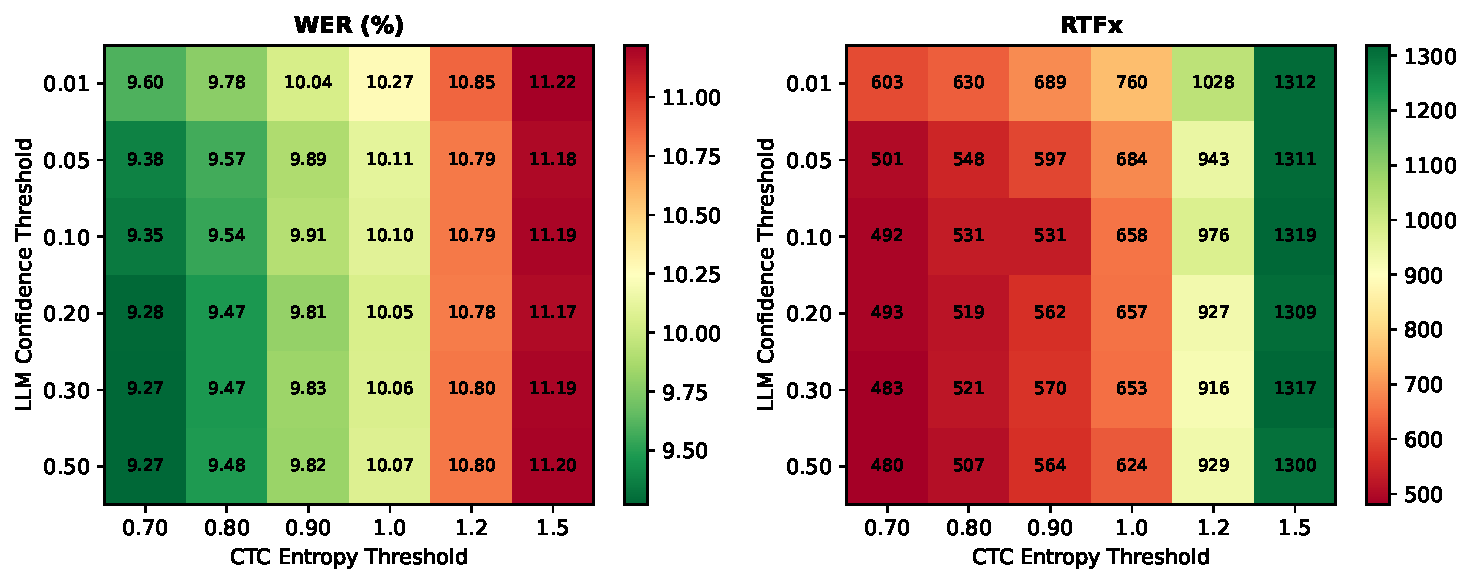
\includegraphics[width=8cm]{figures/sweep_v24_2d_heatmap.pdf}
\caption{Influence of acceptance thresholds $\tau_{CTC}$ and $\tau_{SLM}$ on word error rate and inverse real-time factor for Earnings-22.}
\label{fig:heatmap}
\end{figure}                                                        

In Figure~\ref{fig:heatmap} we study the influence of the CTC and LLM verification thresholds on WER and RTFx for the Earnings-22 corpus and conclude that $\tau_{CTC}$ has a much stronger influence on the operating point. Therefore, we fix $\tau_{SLM}=0.1$ throughout the experiments and only vary $\tau_{CTC}\in[0.7,3.0]$ except for the high accuracy settings in Table~\ref{tab:results} where $\tau_{SLM}=0.2$.  

\subsection{Verification pass ablation study}
Here we answer the question if both verification stages are necessary for optimal performance across the entire WER-RTFx spectrum. Concretely, we contrast using both CTC and LLM acceptance passes with using a single verification stage (either CTC or LLM). The results from Figure~\ref{fig:ablation} suggest that deactivating the CTC acceptance pass (i.e. directly sending the CTC hypotheses to LLM verification) has similar performance to the baseline in the high accuracy regime but has substantially lower RTFx at the high throughput end. Conversely, deactivating the LLM verification pass (i.e. using only CTC entropy acceptance and full AR fallback for rejected samples) cannot reach the lowest WER in the high accuracy regime (5.75\% vs. 5.58\%) but does match the baseline curve for high RTFx. The proposed method using both verification steps dominates across most of the range and achieves the best Pareto frontier.

\begin{figure}[!t]
\centering
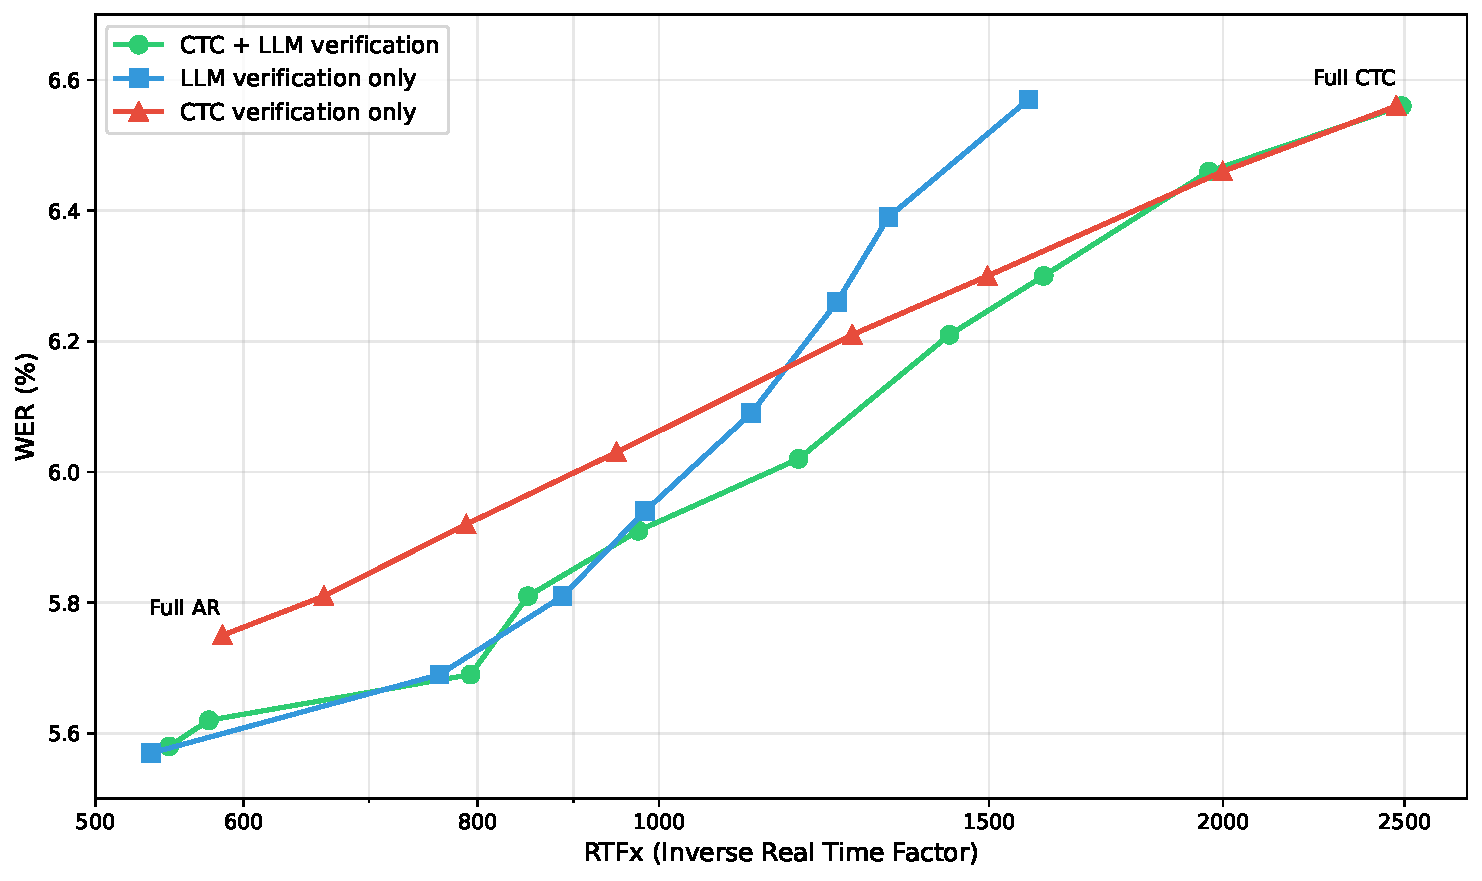
\includegraphics[width=8cm]{figures/verification_comparison.pdf}
\caption{Ablation study of verification passes: green = CTC followed by LLM; blue = LLM verification; red = CTC verification. Results are reported on the ESB/Open ASR test sets.}
\label{fig:ablation}
\end{figure}                                                        

\subsection{LLM verification improves accuracy over full AR}
As can be seen from the results in Table~\ref{tab:results} and Figure~\ref{fig:ablation}, the LLM verification stage of the CTC hypotheses reduces WER across all corpora compared to full auto-regressive decoding. We surmise that this is due to a system combination effect between CTC and SLM which make complementary recognition errors. In Table~\ref{tab:examples} we show some examples where the LLM-verified CTC hypotheses are more accurate than those obtained with full AR decoding. It is apparent that the AR outputs tend to be more fluent but not always faithful to the acoustics which is a well-known problem for encoder-decoder models such as Whisper called language model bias~\cite{koenecke2024careless}.

\begin{figure}[!t]
\centering
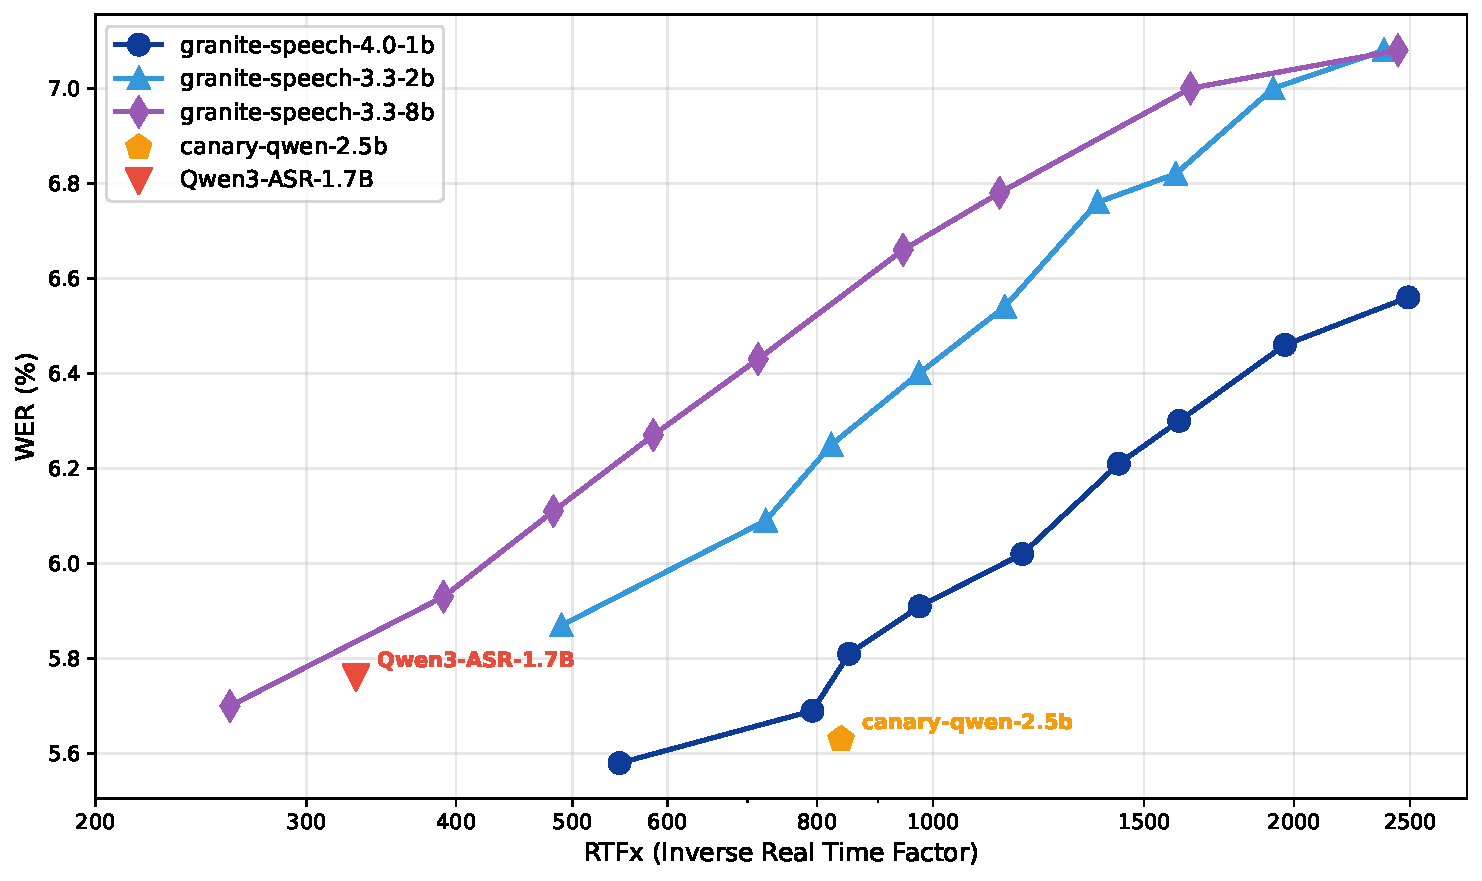
\includegraphics[width=8cm]{figures/wer_vs_rtfx_v24_nar.pdf}
\caption{WER and RTFx comparison between granite-speech and leading SLMs on the Open ASR test sets (all on 1 H100).}
\label{fig:comparison}
\end{figure}     

\begin{table}
\centering
\caption{Examples where LLM-verified CTC hypotheses are more accurate than full AR decoding.
Errors are shown in \textbf{bold}.}
\label{tab:examples}
\tiny
\begin{tabular}{l}
\toprule
\textbf{AMI} \\
\midrule
\texttt{REF: so if you can work on it that and then ~~like no actually not} \\
\texttt{CTC: so if you can work on it that and then ~~like no actually not} \\
\texttt{AR:~ so if you can work on \textbf{**} that and then \textbf{i} like no actually not} \\
\midrule
\textbf{LibriSpeech test-other} \\
\midrule
\texttt{REF: and i~tanquam ~sponsus} \\
\texttt{CTC: and i~tanquam ~spons\textbf{i}s} \\
\texttt{AR:~ and i~tan\textbf{t}quam spons\textbf{i}s} \\
\midrule
\texttt{REF: what chucked him off yonder} \\
\texttt{CTC: what \textbf{tr}ucked him off yonder} \\
\texttt{AR:~ what \textbf{tr}ucked \textbf{em}~~off yonder} \\
\midrule
\textbf{Voxpopuli} \\
\midrule
\texttt{REF: business~~ is ~demanding workers are demanding we are demanding do more} \\
\texttt{CTC: business~~ is ~demanding workers are demanding we are demanding do more}\\
\texttt{AR:~ business\textbf{es} \textbf{are} demanding workers are demanding we are demanding do more}\\
\midrule
\texttt{REF: i declare ~~particular interest on this matter} \\
\texttt{CTC: i declare ~~particular interest \textbf{in} this matter} \\
\texttt{AR:~ i declare \textbf{a} particular interest \textbf{in} this matter} \\

\bottomrule
\end{tabular}
\end{table}

\subsection{Detailed results}
In Table~\ref{tab:results}, we report WER and RTFx results for granite-speech-4.0-1b on the ESB/Open ASR English test sets as well as on two multilingual corpora (CommonVoice 17.0 and MLS). We observe that, in the high accuracy regime, SSD outperforms full AR across all corpora with no loss in throughput. The improvement in accuracy stems from a low CTC acceptance rate (column \%C) and a high LLM acceptance rate of 40-50\% of CTC hypotheses (column \%L). In the high RTFx regime, we accelerate inference by a factor of 4.4 on Open ASR with a 12\% degradation in WER by having close to 100\% CTC gating. As for runtime, Figure~\ref{fig:timing} shows that the encoder and fallback AR stages are the most time-consuming in the high accuracy regime.

Finally, in Figure~\ref{fig:comparison}, we compare three granite-speech models (3.3-2b, 3.3-8b and 4.0-1b) with SSD against the top 2 closest competitors (canary-qwen-2.5b~\cite{chen2024salm,sekoyan2025canary} and qwen3-asr-1.7b~\cite{shi2026qwen3asrtechnicalreport}). To ensure fair RTFx comparisons, we have run the Open ASR benchmark for the latter ourselves using the official HuggingFace evaluation harnesses provided for those models. 

\section{Conclusion and future work}
\label{sec:conclusion}
We have shown that both accuracy and inference speed of speech-aware LLMs can be improved by using fast CTC encoder drafts computed non-autoregressively. Accuracy is improved by LLM verification of acoustically-grounded CTC hypotheses which can mitigate errors due to language modeling bias. Throughput is improved by accepting high-confidence CTC drafts. Importantly, this is achieved without retraining the SLM or having to provide a separate draft model but by simply using the CTC head of the encoder for rapid transcription and gating and the LLM for verification and fallback AR decoding. 
Future work will look at training the encoder jointly with the LLM specifically for speculation (high LLM acceptance rate while maintaing accuracy) and at applying some of these ideas to reduce latency for real-time conversational applications.

\section{Generative AI Use Disclosure}
The code used in the experiments was written with help from a coding assistant (Claude by Anthropic). The experiments were run manually and results were manually verified. Generative AI was also used in the formatting of tables and in figure design. The rest of the paper was manually written with no AI proofreading or editing. The authors assume full responsibility and accountability for the content of this submission.

\bibliographystyle{IEEEtran}
\bibliography{mybib}

\end{document}

\subsection{General guidelines}

Authors are encouraged to describe how their work relates to prior work by themselves and by others, and to make clear statements about the novelty of their work. This may require careful wording to avoid unmasking the identity of the authors in the version submitted for review (guidance in Section \ref{section:doubleblind}). All submissions must be compliant with the \textbf{ISCA Code of Ethics for Authors}, the \textbf{Pre-prints Policy}, and the \textbf{Conference Policy}. These can be found on the conference website under the ``For authors'' section.

\subsubsection{Originality}

All papers submitted to Interspeech 2026 must be original contributions that are not currently submitted to any other conference, workshop, or journal, nor will be submitted to any other conference, workshop, or journal during the review process of Interspeech 2026. Cross-checks with submissions from other conferences will be carried out to enforce this rule.

\subsubsection{Generative AI tools}

All (co-)authors must be responsible and accountable for the work and content of the paper, and they must consent to its submission. Generative AI tools cannot be a co-author of the paper. They can be used for editing and polishing manuscripts, but should not be used for producing a significant part of the manuscript.
\blue{The use of generative AI tools should be acknowledged in a subsection titled Generative AI Use Disclosure between the Acknowledgments of the References.}






\subsubsection{\blue{List of authors}}

{\color{blue}

When preparing the author list, please observe the following guidelines:
\begin{itemize}
\item Clearly list all authors who have made a significant contribution to the work.
\item The maximum number of authors in the author list is 20. If there are more than 20 contributing authors, the additional authors should be acknowledged in a footnote or in the acknowledgments section.
\item The use of ORCID identifiers for authors is optional but strongly encouraged. It will become mandatory in the future.
\item Submissions must be anonymous: author names and affiliations must not appear in the manuscript during review. However, the full list of authors (and affiliations) must be entered in the submission platform when submitting the paper for review.
\item During the development phase of the paper, authors may keep the full (non-anonymized) list of authors and affiliations in their working copy to verify layout and space constraints. Anonymization should be applied at the final stage before generating the version for submission.
\end{itemize}
}




\subsubsection{Conference theme}

\blue{The theme for Interspeech 2026, "Speaking Together," reflects our dedication to the celebration of all voices. This conference aims to showcase groundbreaking work in under-resourced languages, atypical speech and initiatives to improve access to speech technology for all speakers.}

\subsubsection{Participation in reviewing}

Interspeech uses peer review to evaluate submitted manuscripts. At least one co-author of each paper should be volunteering to review for the Interspeech conference. If you are eligible, but not yet a reviewer for ISCA conferences, you should sign up at

\begin{center}
    \url{https://isca-speech.org/Reviewing}
\end{center}
using the same email address as in your CMT account.
The eligibility criteria can be located through the above link. Papers for which no author qualifies as ISCA reviewer do not have to follow this guideline. During submission, authors should indicate the email of any co-authors who should be added to the reviewer database.

\subsubsection{Accessibility recommendations}

\blue{Authors are encouraged to have their papers fulfill specific requirements relating to \textbf{figures} (see Section \ref{sec:figures}) and \textbf{tables} (see Section \ref{sec:tables}).}


\subsubsection{Scientific reporting check list}

The following checklist will be part of the submission form and includes a list of guidelines we expect Interspeech 2026 papers to follow. A compact version of the checklist is available under ``For authors'' section. Not every point in the check list will be applicable to every paper. Ideally, all guidelines that do apply to a certain paper should be satisfied. Nevertheless, not satisfying a guideline that applies to your paper is not necessarily grounds for rejection.

\begin{enumerate}

\item Claims and limitations - for all papers
\begin{itemize}

\item The paper clearly states what claims are being investigated, and why.
\item The novelties are clearly explained.
\item The main claims made in the abstract and introduction accurately reflect the paper’s contributions and scope.
\item The limitations of your work are described.
\item The relevant assumptions made in your work are stated in the paper.
\end{itemize}

\item If models are used, the paper includes information about the following:
\begin{itemize}
    \item Justification for each selected model, algorithm, or architecture.
    \item Sufficient details of the model (architecture), including reference(s) to prior literature.
\end{itemize}

\item If data sets are used, the paper includes information about the following:
\begin{itemize}
\item Relevant details such as languages, audio duration distribution, number of examples, and label distributions, or a reference where that information can be found.
\item Details of train/validation (development)/test splits. Ideally, the lists should be released with the supplementary material if not already publicly available.
\item Explanation of all pre-processing steps, including any criteria used to exclude samples, if applicable.
\item Reference(s) to all data set(s) drawn from the existing literature.
\item For newly collected data, a complete description of the data collection process, such as subjects, instructions to annotators and methods for quality control and a statement on whether ethics approval was necessary.
\end{itemize}

\item If using non-public data sets or pre-trained models:
\begin{itemize}
\item The paper includes a discussion on the reason/s for using non-public data sets.
\item Full details of the dataset are included in the paper to enable comparison to similar data sets and tasks.
\item For papers that use publicly available, pre-trained (e.g. foundational or self-supervised) models, link to the model is provided. For papers that use non-public pre-trained models, description of the data (including quantity) used for training that model is provided.
\end{itemize}


\item If reporting experimental results, the paper includes:
\begin{itemize}
\item An explanation of evaluation metrics used.
\item An explanation of how models are initialized, if applicable.
\item Some measure of statistical significance of the reported gains or confidence intervals.
\item A description of the computing infrastructure used and the average runtime for each model or algorithm (e.g. training, inference etc).
\item The number of parameters in each model.
\end{itemize}

\item If hyperparameter search (including choice of architecture or features and any other development decision) was done, the paper includes:
\begin{itemize}
\item Final results on a held-out evaluation set not used for hyperparameter tuning.
\item Hyperparameter configurations for best-performing models.
\item The method for choosing hyperparameter values to explore, the range of the hyperparameter values, and the criterion used to select among them.
\end{itemize}

\item If source code is used:
\begin{itemize}
\item The code is or will be made publicly available and/or sufficient details are included in the paper for the work to be reproduced.
\item For publicly available software, the corresponding version numbers and links and/or references to the software.
\end{itemize}

\end{enumerate}

For any paper that uses machine learning, we encourage authors to provide statistical significance tests and follow well-established processes for evaluating any statistical or machine learning model. \blue{McNemar’s test \cite{mcnemar1947} is one of the most popular tests used in the literature to report statistical significance (e.g., \cite{fiscus1997post, chollet1995evaluation, williams2008exploiting, busch2025multilingual, lin2025voice, lee2025performance}). Other examples include ANOVA \cite{allbert2025evaluating}, adding error bars~\cite{miller2024addingerrorbarsevals}, and bootstrapping approaches~\cite{ferrer2024goodpracticesevaluationmachine, url2025}.}

\subsection{Double-blind review}
\label{section:doubleblind}

Interspeech~2026 uses double-blind review to support the integrity of the review process.

\subsubsection{Version submitted for review}

The manuscript submitted for review must not include any information that might reveal the authors' identities or affiliations. This also applies to the metadata in the submitted PDF file (guidance in Section \ref{section:pdf_sanitise}), uploaded multimedia and online material (guidance in Section \ref{section:multimedia}).

Take particular care to cite your own work in a way that does not reveal that you are also the author of that work. For example, do not use constructions like ``In previous work [23], we showed that \ldots''. Instead use something like ``Jones et al. [23] showed that \ldots''.

Acknowledgements should not be included in the version submitted for review.

{\color{blue}
For \LaTeX{} users, make sure to activate the review mode of the template by uncommenting the line \verb|\documentclass{Interspeech}| and commenting the line \verb|\documentclass[cameraready]{Interspeech}| at the beginning of the template.}

Papers that reveal the identity of the authors will be rejected without review.
Note that the full list of authors must still be provided in the online submission system, since this is necessary for detecting conflicts of interest.

\subsubsection{Camera-ready version}

Authors should include names and affiliations in the final version of the manuscript, for publication.

{\color{blue}
For \LaTeX{} users, make sure to activate the camera-ready mode of the template by commenting the line \verb|\documentclass{Interspeech}| and uncommenting the line \verb|\documentclass[cameraready]{Interspeech}| at the beginning of the template.
}

Include the country as part of each affiliation. Do not use company logos anywhere in the manuscript, including in affiliations and Acknowledgements. After acceptance, authors may of course reveal their identity in other ways, including: adjusting the wording around self-citations; adding further acknowledgements; updating multimedia and online material. Acknowledgements, if any, should be added in the camera-ready version.

\subsubsection{Pre-prints}
\label{section:preprints}

\blue{Please visit the submission policy under the \textit{For Authors} section of the Interspeech 2026 website (\url{https://interspeech2026.org/}) for a detailed explanation of the policy on pre-prints for this Interspeech. Interspeech no longer enforces an anonymity period for submissions published in archive repositories.  While uploading a version online is permitted, your official submission to Interspeech must not contain any author-identifying information.}



\section{Format}

\subsection{Layout}

Authors should observe the following specification for page layout by using the provided template. Do not modify the template layout! Do not reduce the line spacing!

\subsubsection{Page layout}

\begin{itemize}
\item Paper size must be DIN A4.
\item Two columns are used except for the title section and for large figures or tables that may need a full page width.
\item Left and right margin are \SI{20}{\milli\metre} each.
\item Column width is \SI{80}{\milli\metre}.
\item Spacing between columns is \SI{10}{\milli\metre}.
\item Top margin is \SI{25}{\milli\metre} (except for the first page which is \SI{30}{\milli\metre} to the title top).
\item Bottom margin is \SI{35}{\milli\metre}.
\item Text height (without headers and footers) is maximum \SI{235}{\milli\metre}.
\item Page headers and footers must be left empty.
\item No page numbers.
\item Check indentations and spacing by comparing to the example PDF file.
\end{itemize}

\subsubsection{Section headings}

Section headings are centred in boldface with the first word capitalised and the rest of the heading in lower case. Sub-headings appear like major headings, except they start at the left margin in the column. Sub-sub-headings appear like sub-headings, except they are in italics and not boldface. See the examples in this file. No more than 3 levels of headings should be used.

\subsubsection{Fonts}

Times or Times Roman font is used for the main text. Font size in the main text must be 9 points, and in the References section 8 points. Other font types may be used if needed for special purposes. \LaTeX\xspace users should use Adobe Type 1 fonts such as Times or Times Roman, which is done automatically by the provided \LaTeX\xspace class. Do not use Type 3 (bitmap) fonts. Phonemic transcriptions should be placed between forward slashes and phonetic transcriptions between square brackets, for example \textipa{/lO: \ae nd O:d3/} vs. \textipa{[lO:r@nO:d@]}, and authors are encouraged to use the terms `phoneme' and `phone' correctly \cite{moore19_interspeech}.


\subsubsection{Hyperlinks}

For technical reasons, the proceedings editor may strip all active links from the papers during processing. URLs can be included in your paper if written in full, e.g., \url{https://www.interspeech2026.org/}. The text must be all black. Please make sure that they are legible when printed on paper.


\subsection{Figures}\label{sec:figures}

Figures must be centred in the column or page. Figures which span 2 columns must be placed at the top or bottom of a page.
Captions should follow each figure and have the format used in Figure~\ref{fig:speech_production}. Diagrams should preferably be vector graphics. Figures must be legible when printed in monochrome on DIN A4 paper; a minimum font size of  8 points for all text within figures is recommended. Diagrams must not use stipple fill patterns because they will not reproduce properly in Adobe PDF. See \textit{APA Guidelines regarding the use of color in Figures} (\url{https://apastyle.apa.org/style-grammar-guidelines/tables-figures/colors}).

From an accessibility standpoint, please ensure that your paper remains coherent for a reader who cannot see your figures. Please make sure that:
    \begin{itemize}
        \item all figures are referenced in the text.
        \item figures are fully explained either in text, in their caption, or in a combination of the two.
        \item instead of visualizing differences between areas in your figures only by color, those differences can also be illustrated by using different textures or patterns.
        \item all text, including axis labels, is at least as large as the content text surrounding the figures.
        \item \blue{We encourage to use color-blind–friendly color palettes (see \url{https://www.color-blindness.com/coblis-color-blindness-simulator/})}
    \end{itemize}


\subsection{Tables}\label{sec:tables}

An example of a table is shown in Table~\ref{tab:example}. The caption text must be above the table. Tables must be legible when printed in monochrome on DIN A4 paper; a minimum font size of 8 points is recommended. 

From an accessibility standpoint, please make sure that:
    \begin{itemize}
        \item tables are not images.
        \item all table headings are clearly marked as such, and are distinct from table cells.
        \item all tables are referenced in the text.
    \end{itemize}

\begin{table}[th]
  \caption{This is an example of a table}
  \label{tab:example}
  \centering
  \begin{tabular}{ r@{}l  r }
    \toprule
    \multicolumn{2}{c}{\textbf{Ratio}} &
                                         \multicolumn{1}{c}{\textbf{Decibels}} \\
    \midrule
    $1$                       & $/10$ & $-20$~~~             \\
    $1$                       & $/1$  & $0$~~~               \\
    $2$                       & $/1$  & $\approx 6$~~~       \\
    $3.16$                    & $/1$  & $10$~~~              \\
    $10$                      & $/1$  & $20$~~~              \\
    \bottomrule
  \end{tabular}

\end{table}



\subsection{Equations}

Equations should be placed on separate lines and numbered. We define
%
\begin{align}
  x(t) &= s(t') \nonumber \\
       &= s(f_\omega(t))
\end{align}
%
where \(f_\omega(t)\) is a special warping function. Equation \ref{equation:eq2} is a little more complicated.
%
\begin{align}
  f_\omega(t) &= \frac{1}{2 \pi j} \oint_C
  \frac{\nu^{-1k} \mathrm{d} \nu}
  {(1-\beta\nu^{-1})(\nu^{-1}-\beta)}
  \label{equation:eq2}
\end{align}
%



\begin{figure}[t]
  \centering
  
\includegraphics[width=\linewidth]{figure.pdf}
  \caption{Schematic diagram of speech production.}
  \label{fig:speech_production}
\end{figure}


\subsection{Style}

Manuscripts must be written in English. Either US or UK spelling is acceptable (but do not mix them).


\subsubsection{International System of Units (SI)}

Use SI units, correctly formatted with a non-breaking space between the quantity and the unit. In \LaTeX\xspace this is best achieved using the \texttt{siunitx} package (which is already included by the provided \LaTeX\xspace class). This will produce
\SI{25}{\milli\second}, \SI{44.1}{\kilo\hertz} and so on.


\begin{table}[b!]
  \caption{Main predefined styles in Word}
  \label{tab:word_styles}
  \centering
  \begin{tabular}{ll}
    \toprule
    \textbf{Style Name}      & \textbf{Entities in a Paper}                \\
    \midrule
    Title                    & Title                                       \\
    Author                   & Author name                                 \\
    Affiliation              & Author affiliation                          \\
    Email                    & Email address                               \\
    AbstractHeading          & Abstract section heading                    \\
    Body Text                & First paragraph in abstract                 \\
    Body Text Next           & Following paragraphs in abstract            \\
    Index                    & Index terms                                 \\
    1. Heading 1             & 1\textsuperscript{st} level section heading \\
    1.1 Heading 2            & 2\textsuperscript{nd} level section heading \\
    1.1.1 Heading 3          & 3\textsuperscript{rd} level section heading \\
    Body Text                & First paragraph in section                  \\
    Body Text Next           & Following paragraphs in section             \\
    Figure Caption           & Figure caption                              \\
    Table Caption            & Table caption                               \\
    Equation                 & Equations                                   \\
    \textbullet\ List Bullet & Bulleted lists                              \\\relax
    [1] Reference            & References                                  \\
    \bottomrule
  \end{tabular}
\end{table}


\section{Specific information for Microsoft Word}

For ease of formatting, please use the styles listed in Table \ref{tab:word_styles}. The styles are defined in the Word version of this template and are shown in the order in which they would be used when writing a paper. When the heading styles in Table \ref{tab:word_styles} are used, section numbers are no longer required to be typed in because they will be automatically numbered by Word. Similarly, reference items will be automatically numbered by Word when the ``Reference'' style is used.

If your Word document contains equations, you must not save your Word document from ``.docx'' to ``.doc'' because this will convert all equations to images of unacceptably low resolution.

\section{Submissions}

Information on how and when to submit your paper is provided on the conference website.

\subsection{Manuscript}

Authors are required to submit a single PDF file of each manuscript. The PDF file should comply with the following requirements: (a) no password protection; (b) all fonts must be embedded; (c) text searchable (do ctrl-F and try to find a common word such as ``the''), and (d) the document properties do not reveal the identity or username. The conference organisers may contact authors of non-complying files to obtain a replacement. Papers for which an acceptable replacement is not provided in a timely manner will be withdrawn.

\subsubsection{Embed all fonts}

It is \textit{very important} that the PDF file embeds all fonts!  PDF files created using \LaTeX, including on \url{https://overleaf.com}, will generally embed all fonts from the body text. However, it is possible that included figures (especially those in PDF or PS format) may use additional fonts that are not embedded, depending how they were created.

On Windows, the bullzip printer can convert any PDF to have embedded and subsetted fonts. On Linux \& MacOS, converting to and from Postscript will embed all fonts:
\\

\noindent\textsf{pdf2ps file.pdf}\\
\noindent\textsf{ps2pdf -dPDFSETTINGS=/prepress file.ps file.pdf}


\subsubsection{Sanitise PDF metadata}
\label{section:pdf_sanitise}

Check that author identity is not revealed in the PDF metadata. The provided \LaTeX\xspace class ensures this. Metadata can be inspected using a PDF viewer.


\subsection{Optional supplementary material or links to online material}
\label{section:multimedia}

\subsubsection{Supplementary material}
\label{section:supplementary}

Interspeech offers the option of submitting supplementary material.
These files are meant for code, data or audio-visual illustrations that cannot be conveyed in text, tables and graphs. Just as with figures used in your manuscript, make sure that you have sufficient author rights to all other materials that you submit. This material will be available to reviewers and committee members for evaluating the paper, but it will not be published with the paper or accessible in the archives. To make material available for future readers, please use online resources (see section \ref{section:repos}). Supplementary material is intended to support the reviewers in assessing the paper; however, the paper should be understandable on its own. Reviewers may choose to examine the supplementary material but are not required to do so.

In line with the double-blind review policy, make sure that the supplementary material is anonymised. Unless strictly necessary, avoid to provide code at this step, which is usually harder to anonymise.

Your supplementary material must be submitted in a single ZIP file limited to 100 MB for each separate paper. Within the ZIP file you can use folders to organise the files. In the ZIP file you should include a \texttt{README.txt} or \texttt{index.html} file to describe the content. In the manuscript, refer to a supplementary file by filename. Use short file names with no spaces.

\subsubsection{Online resources such as web sites, blog posts, code, and data}
\label{section:repos}

It is common for manuscripts to provide links to web sites (e.g., as an alternative to including a ZIP file as supplementary material), code repositories, data sets, or other online resources. Provision of such materials is generally encouraged; however, they should not be used to circumvent the limit on manuscript length. In particular, reviewers will not be required to read any content other than the main manuscript.

Links included in the version submitted for review should not reveal the identity or affiliation of the authors. If this is not possible, then the links should not be provided in the version submitted for review, but they can be added in the final version of the paper, if accepted. A placeholder can be included in the paper with a text like: ``[to ensure author anonymity, the link to the resource will be added after the review process]''. Links and repositories provided for review should be anonymous. In particular, names in repositories are forbidden.

Authors are encouraged to group any supplementary material in a single repository. If the paper is accepted, authors will have the option to include a single link to this repository in the paper's metadata on ISCA Archives. For that purpose, the link must be a DOI link. Free DOI links can for instance be obtained through Zenodo, with additional guidance available in GitHub Docs (\url{https://docs.github.com/en/repositories/archiving-a-github-repository/referencing-and-citing-content})

\section{Discussion}

Authors must proofread their PDF file prior to submission, to ensure it is correct. Do not rely on proofreading the \LaTeX\xspace source or Word document. \textbf{Please proofread the PDF file before it is submitted.}

\section{Acknowledgments}

{\color{blue}Acknowledgments should be included only in the camera-ready version, not in the version submitted for review. For regular papers, pages 5 and 6, and for long papers, pages 9 and 10, are reserved exclusively for acknowledgments, disclosures of the use of generative AI tools, and references. No other content may appear on these pages. Any appendices must be contained within the first four pages for regular papers and within the first eight pages for long papers.

Acknowledgments and references may begin on an earlier page if space permits.}

\ifcameraready
     The Interspeech 2026 organizers
\else
     The authors
\fi
would like to thank ISCA and the organizing committees of past Interspeech conferences for their help and for kindly providing the previous version of this template.




{\color{blue}
\section{Generative AI Use Disclosure}
The extent of Generative AI use must be disclosed. This section may be in the 5th or 6th pages of regular papers, or the 9th or 10th pages of long papers.  ISCA policy says: \textit{All (co-)authors must be responsible and accountable for the work and content of the paper, and they must consent to its submission. Any generative AI tools cannot be a co-author of the paper. They can be used for editing and polishing manuscripts, but should not be used for producing a significant part of the manuscript}.}



\section{Reference Format}

{\color{blue}It is ISCA policy that papers submitted to Interspeech should refer to peer-reviewed publications. References to non-peer-reviewed publications (including public repositories such as arXiv, Preprints, and HAL, software, and personal communications) should only be made if there is no peer-reviewed publication available, and should be kept to a minimum.

References should be in standard IEEE format (follows the IEEEtran format), numbered in order of appearance, for example \cite{Davis80-COP} is cited before \cite{Rabiner89-ATO}. For longer works such as books, provide a single entry for the complete work in the References, then cite specific pages \cite[pp.\ 417--422]{Hastie09-TEO} or a chapter \cite[Chapter 2]{Hastie09-TEO}. Multiple references may be cited in a list \cite{Smith22-XXX, Jones22-XXX}.}


\bibliographystyle{IEEEtran}
\bibliography{mybib}

\end{document}

%%% Local Variables:
%%% mode: LaTeX
%%% TeX-master: t
%%% End:
